\section{Design of an FPGA-based accelerator integrating structured sparse DSC} \label{sec:design}
As previously said,  the aim of this section is to develop a pruning scheme for \acrshort{cnn} model (MobileNetV2) and an algorithm able to support it. First we detail the pruning scheme used and the gain obtained by applying the pruning. Second, we describe the algorithm to perform the convolution using weights pruned with the scheme. Finally, we analyse the loops of the convolution in order to determine the design of the \acrshort{pe} that will perfom the operation.
%
\subsection{Pruning scheme} \label{subsec:pscheme}
%
\acrshort{dsc} is composed of two types of convolution: depthwise and pointwise convolutions. We have decided to apply pruning on the pointwise filters for the following reasons:
%
\begin{itemize}
    \item In MobileNet and MobileNetV2, most of the operations are done in the pointwise convolutions \cite{zhang_channel_2019, tu_pruning_2019}. So it is the operation where the reduction of the computational complexity would be the most relevant.
    \item As each kernel of pointwise filter is a vector of size $1 \times 1  \times Nif$, we therefore have to prune in the channel axis. This scheme has been proven to be successful by \textcite{kang_accelerator-aware_2020}.
    \item The pruning scheme can be applied to each $1 \times 1$ convolution in the network.
\end{itemize}
%
As mentionned above, we decided to develop a pruning scheme inspired by the methodology of \textcite{kang_accelerator-aware_2020} which performs a channel-axis pruning.

Ideally, without pruning, each \acrshort{pe} performing a pointwise convolution, fetches $N_{if}$ weights and their corresponding input pixels (pointwise convolution only convolve pixels in the channel-axis). Then each weight is convolved with its corresponding pixel. If we apply an unstructured pruning, we simply have to convolve the non-pruned weights with their corresponding pixels. However, as the resources of the \acrshort{fpga} are limited, the \acrshort{pe} can only load $N_{par} \leq N_{if}$ weights and pixels (which corresponds to a \textbf{fetching group}; each input \acrshort{fm} and kernel are composed of $N_{gr}$ fetching groups). This causes several issues to the unstructured pruning of the pointwise kernel, as pointed out by \cite{kang_accelerator-aware_2020}.

\begin{figure}
    \centering
    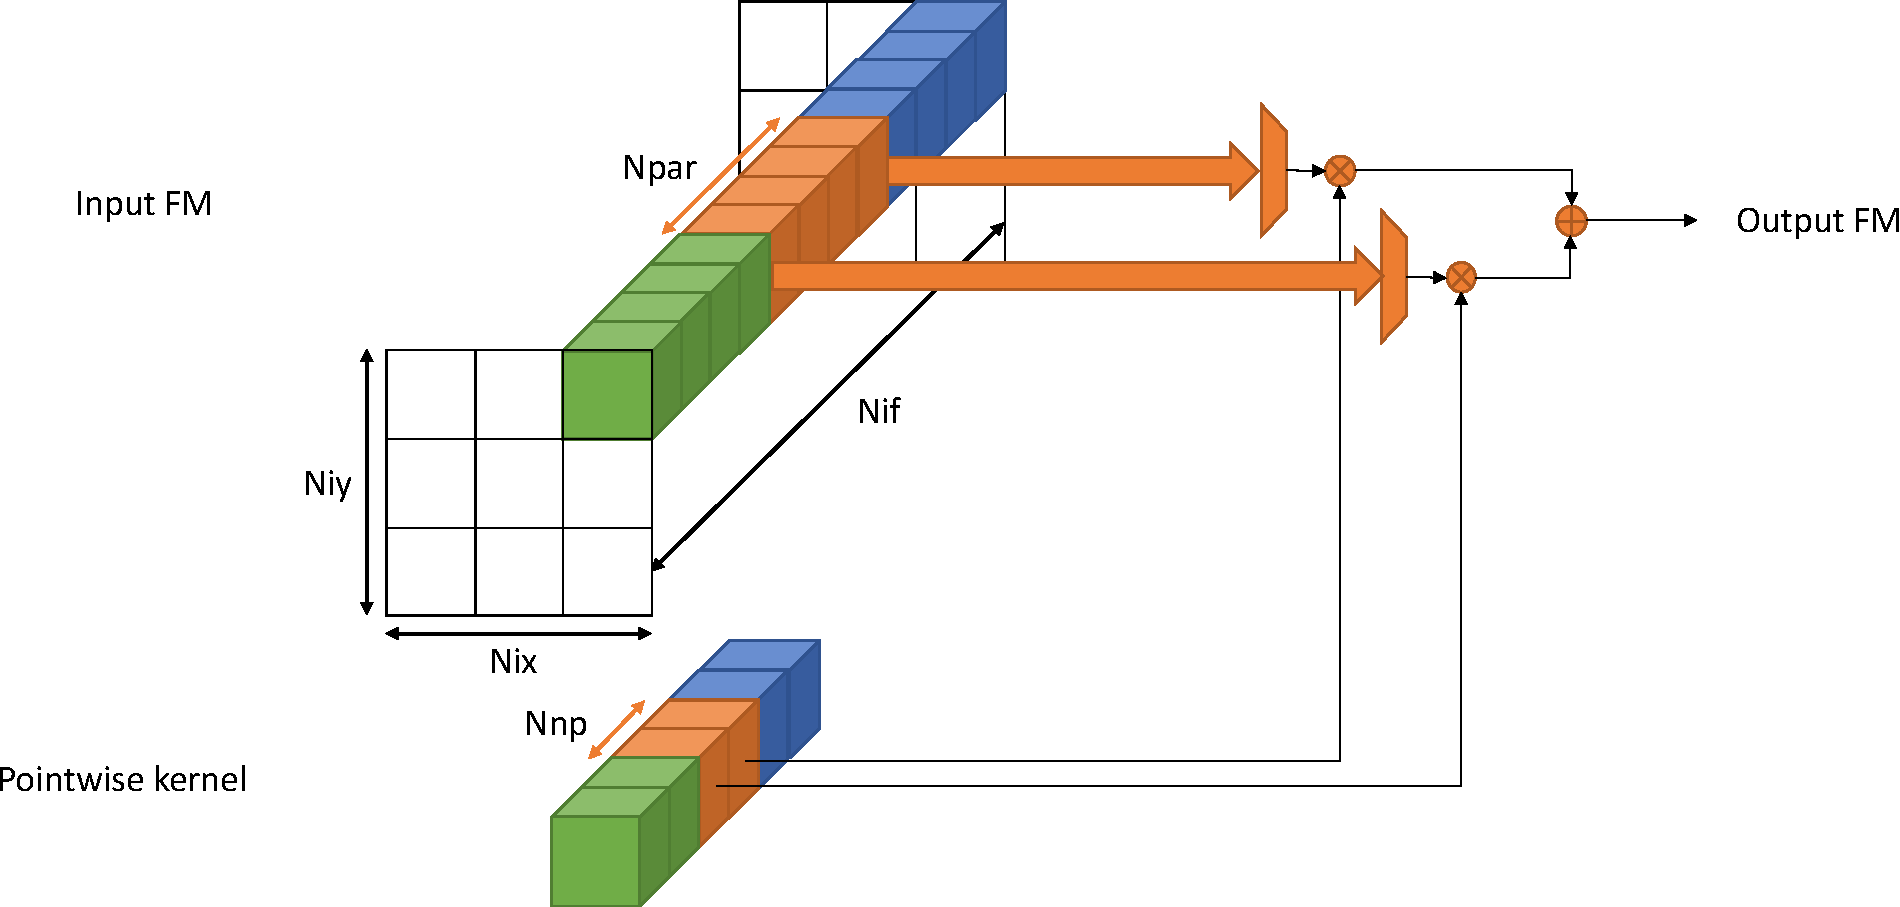
\includegraphics[width=\textwidth]{pruningscheme.pdf}
    \caption{Process of convolution with a sparse pointwise kernel, inspired from \cite{kang_accelerator-aware_2020}}
    \label{fig:prunedwg}
\end{figure}
%
First, it can cause misalignement between the weight and pixel fetching groups. Indeed if we prune the first $N_{par}$ weights in the kernel, the first pixel fetching group is useless. Second, there can be a load-imbalance problem that can occur between two \acrshort{pe}s if the number of weights between the two kernels is different. To solve these problems, the solution proposed by \cite{kang_accelerator-aware_2020} is to align pixel and weight fetching groups. We also constrain the number of non-pruned weights in each fetching group to be the same number, called $N_{np}$, as illustrated in Figure \ref{fig:prunedwg}. Therefore, it solves also the load-imbalance problem and can be applied to each $1 \times 1$ kernel.

%
\begin{table}
    \center
    \begin{tabular}{|c|c|c|}
        \hline
        $N_{par}$ & The input pixel fetching group size. & $N_{par} \leq N_{if}$ \\
        \hline
        $N_{np}$  & The pointwise weight fetching group size. & $N_{np} \leq N_{par}$ \\
        \hline
        $N_{gr}$  & The number of fetching groups & $N_{gr} = \left\lceil \frac{N_{if}}{N_{par}} \right\rceil $ \\
        \hline
        $\alpha$  & The pruning ratio & $\alpha = \frac{N_{np}}{N_{par}}  $ \\
        \hline
    \end{tabular}
    \caption{Pruning parameters}
    \label{tab:pr_param}
\end{table}
%
To summarise, each depthwise kernel is composed of $N_{gr}$ fetching groups of $N_{np}$ weights. Each group corresponds to a pixel fetching group of size $N_{par}$. The pruning parameters are defined in Table \ref{tab:pr_param}. We should add that this pruning scheme is not the same as \textit{channel pruning} since we do not constrain the same weights to be pruned in each group. Therefore, I have not considered the pruning of the pointwise filter associated with the pruning of a weight in each kernel. We have then proposed a pruning-scheme that is not coarse-grained (channel pruning), satisfying first design objective: \textbf{\textquote{The pruning scheme is as fine-grained as possible}}.
%
\subsubsection{Reduction factors}
%
We can now evaluate the reduction factors of the sparse \acrshort{dsc} compared with the \acrshort{dsc} without pruning and the standard convolution.

We consider that the size of the input feature map of the pointwise convolution is $N_{ix}  \times N_{iy} \times N_{if}$, the size of the depthwise filter is $N_{kx} \times N_{ky} \times N_{if}$, the size of the non-pruned pointwise convolution $N_{if} \times N_{of}$, the fetching group size is $N_{par}$, and the number of pruned weights is $N_{np}$. The amount of weights $W_{DSC}$ and operations $O_{DSC}$ of the \acrshort{dsc} can be determined using Equation \eqref{eq:dsc_wg} and \eqref{eq:dsc_op} \cite{bai_cnn_2018, liu_fpga-based_2019}.
%
\begin{align}
    W_{DSC} &= N_{kx} \times N_{ky} \times N_{if} + N_{if} + \times N_{of}\\
    O_{DSC} &= N_{ix} \times N_{iy} \times N_{kx} \times N_{ky} \times N_{if} + N_{ix} \times N_{iy} \times N_{if} \times N_{of}
    \label{eq:dsc_op}
\end{align}
%
In a same manner, the amount of weights $W_{PR\_DSC}$ and operations $O_{PR\_DSC}$ of the sparse \acrshort{dsc} can be determined using Equation \eqref{eq:pr_dsc_pr_wg_op}.
%
\begin{align}
    W_{PR\_DSC} &= N_{kx} \times N_{ky} \times N_{if} + \times N_{if} + N_{np} \times N_{gr} \times N_{of}\\
    O_{PR\_DSC} &= N_{ix} \times N_{iy} \times N_{kx} \times N_{ky} \times N_{if} + N_{ix} \times N_{iy} \times N_{gr} \times N_{np} \times N_{of}
    \label{eq:pr_dsc_wg_op}
\end{align}
%
Thus, the weights $F_{Wg}$ and operations $F_{Op}$ reduction factors can be expressed according to Equation \eqref{eq:factor_comp}. The demonstration allowing to find these relations can be found in Appendix \ref{appendix:factor}.

\begin{align}
    F_{Wg} &= \frac{1 + \frac{N_{kx} \times N_{ky}} {N_{of}}} {\alpha + \frac{N_{kx} \times N_{ky}} {N_{of}}}\\
    F_{Op} &= \frac{1 + \frac{N_{kx} \times N_{ky}} {N_{of}}} {\alpha + \frac{N_{kx} \times N_{ky}} {N_{of}}}
    \label{eq:factor_comp}
\end{align}
%
\begin{figure}
    \centering
    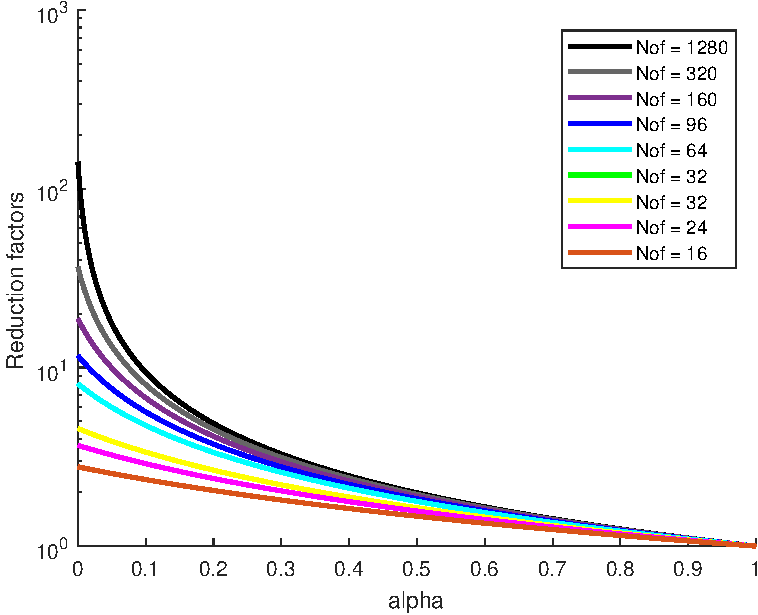
\includegraphics[width=\textwidth]{RedFactor.pdf}
    \caption{Evolution of the reduction factors depending on the pruning ratio and the number of output channel}
    \label{fig:redfacto}
\end{figure}
%
As the reduction factors depend on the pruning ratio $\alpha$, we can illustrate the evolution of the reduction factors depending on this parameter and the different $N_{of}$ of the network. This can be seen on Figure \ref{fig:redfacto}.

For example, if we apply a pruning ratio of $75\%$, the reduction factors compared the \acrshort{dsc} without pruning are between two and four times. If we consider the reduction factor between \acrshort{dsc} and standard convolution is about 9 times \cite{zhang_channel_2019}, the reduction factors between sparse \acrshort{dsc} and standard convolution is between 18 and 36 times. We have therefore validated the second design objective, which is: \textbf{\textquote{The pruning scheme reduces the computational complexity}}.
%
\subsubsection{Compressed format}
%
\begin{figure}
    \centering
    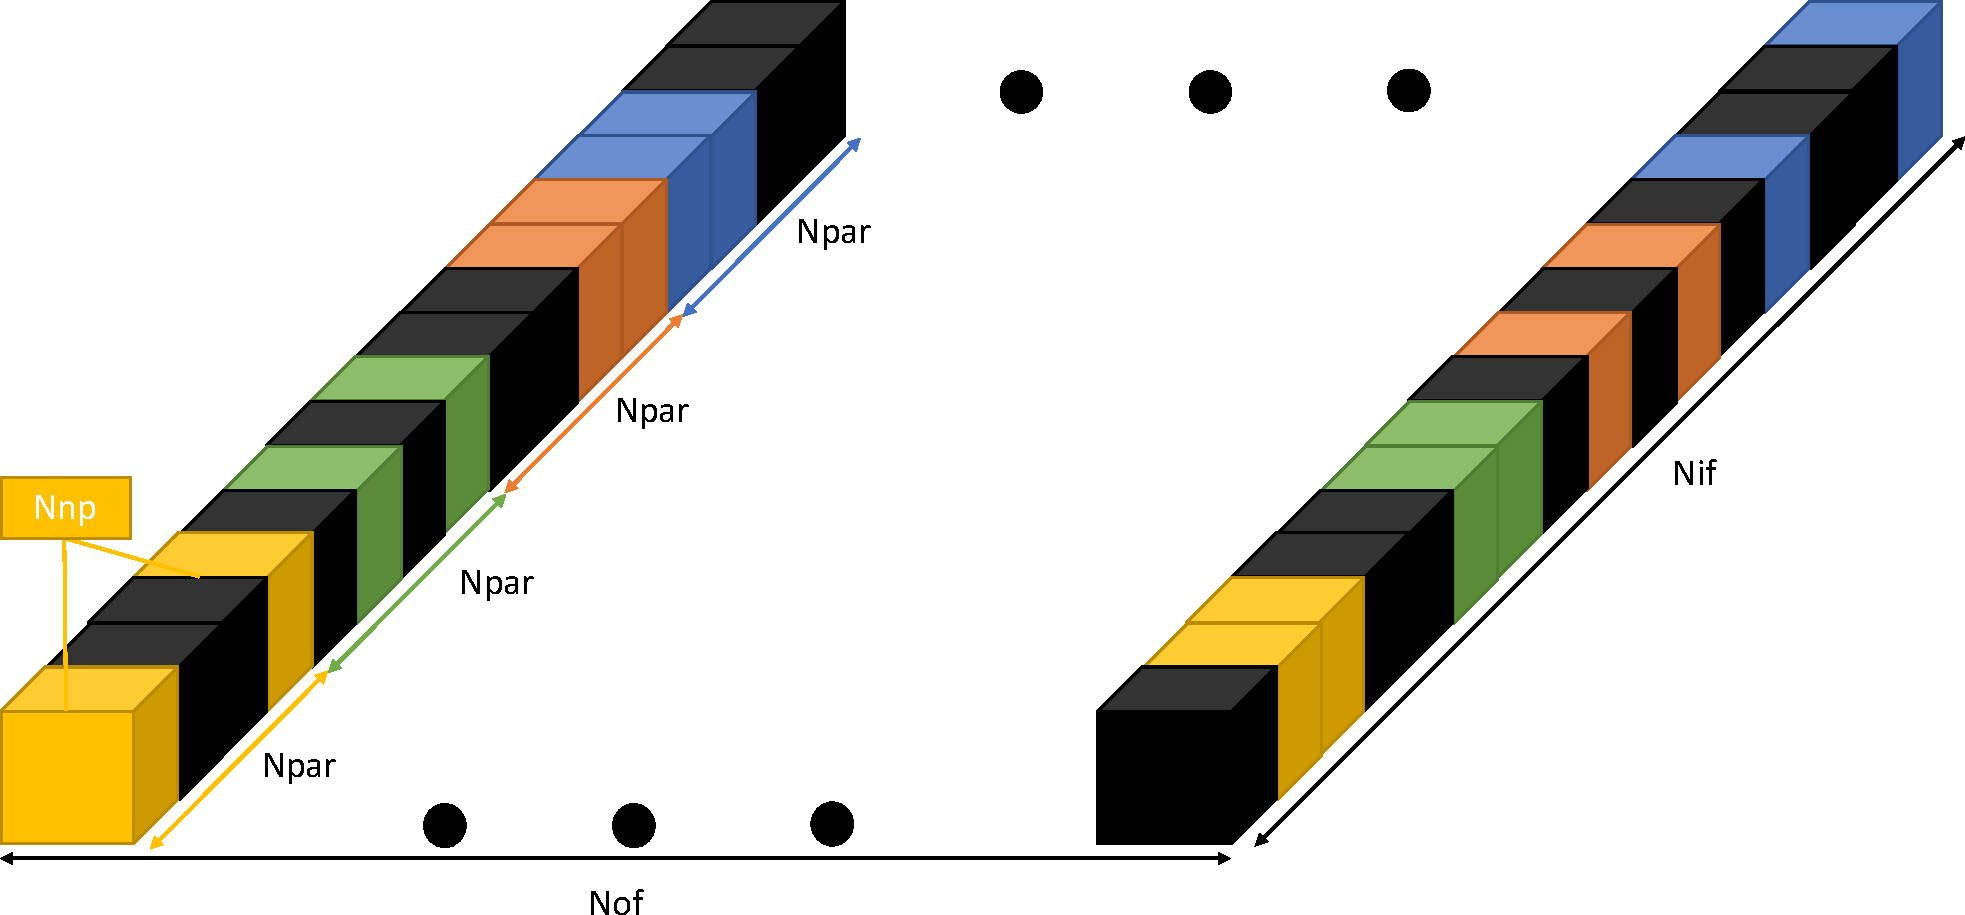
\includegraphics[width=\textwidth]{pruned_wg.pdf}
    \caption{A pointwise kernel after pruning, where black cubes are pruned weights}
    \label{fig:pruned_wg}
\end{figure}
%
After applying the pruning scheme on the pointwise kernels, these kernels become sparse. This means that they contain 0 value weights, as illustrated in Figure \ref{fig:pruned_wg}. Therefore, in order to reduce the memory usage, we should store only the non-pruned weights in a compressed format that allows finding the address of the weights with no extra-overhead.

A conventional storage format for sparse matrix is the \acrfull{csr} \cite{buluc_parallel_2009}. According to \textcite{buluc_parallel_2009}, \textquote{\textit{The compressed sparse row (CSR) format stores the nonzeros (and ideally only the nonzeros) of each matrix row in consecutive memory locations,  and  it  stores  an  index  to  the  first  stored  element of each row}}. In other words, we represent a sparse matrix using three vectors:
%
\begin{itemize}
    \item \textbf{Vector val}: containing all the values of the non-pruned weights.
    \item \textbf{Vector col\_ind}: contains the column indices of the elements in \textbf{val}.
    \item \textbf{Vector row\_ptr}: contains the index of each row in \textbf{val}.
\end{itemize}
%
However, as for \cite{zhu_efficient_2020}, this format can be compressed further thanks to the pruning scheme. Indeed, since the kernels to compress are vectors, we can reduce the storage usage by removing the \textbf{row\_ptr} vector (the vector has only one row). Moreover, we can have a better compression if we reduce the number of bits allocated to represent the column index of a weigth. Indeed, knowing that the weight correponds to a pixel in a fetching group of size $N_{par}$, it is sufficient to store the position of the pixel in that group. As a result, we can reduce the number of bits from $log_2(N_{if})$ to $log_2(N_{par})$, where $N_{par} \leq N_{if}$.

\begin{figure}
    \centering
    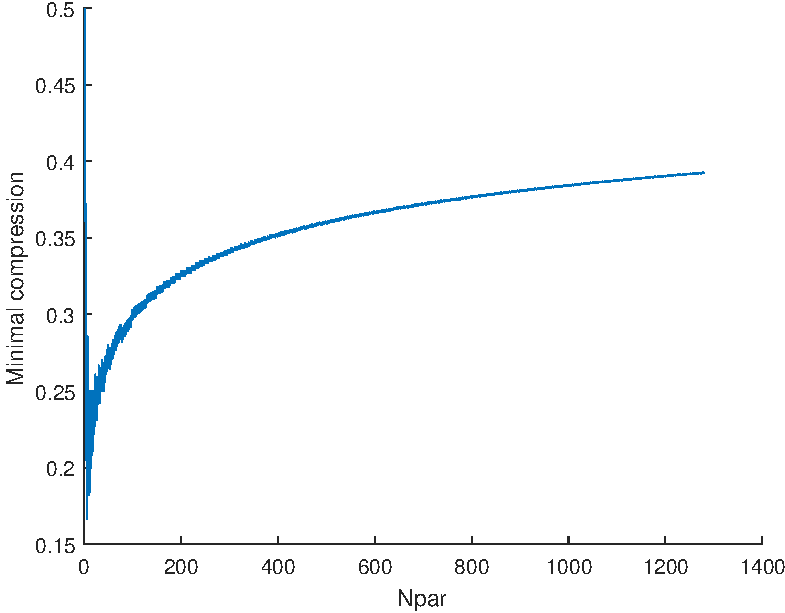
\includegraphics[width=\textwidth]{MinCompr.pdf}
    \caption{Minimal pruning ratio if $BW$ = 16}
    \label{fig:prun_mem}
\end{figure}
%
We compute the minimal pruning ratio required to have a reduction of the memory usage since this compressed format requires an extra position per weight (and hence more memory per weight). The relation between minimal pruning ratio and memory reduction can be found in Equation \eqref{eq:prun_mem} where $BW$ is the bitwidth required to represent the value of a weight. The curve representing the minimal pruning ratio depending on $N_{par}$ is illustrated in Figure \ref{fig:prun_mem}. We can conclude that we need at least a pruning ration of $40\%$ in order to save memory (a fewer pruning ratio can be set if we have a small $N_{par}$). We have therefore validated the third design objective, which is: \textbf{\textquote{The pruning scheme allows a reduction of the memory required to store the weights}}.
%
\begin{equation}
    \alpha < \frac{BW}{ BW + log_2(N_{par})}
    \label{eq:prun_mem}
\end{equation}
%
\subsection{Adding the pruning scheme to MobileNetV2} \label{subsec:mbnv2-pr}
%
As we have seen how the weights of a $1 \times 1$ kernel are pruned and explained the compressed format of the kernels, we present in this section how to integrate the proposed pruning scheme into MobileNetV2. In MobileNetV2, the \acrshort{dsc} layer is included into a larger building block, the \textit{inverted residual block} (see Section \ref{subs:mbv2}). It means that the \acrshort{dsc} follows a $1 \times 1$ convolution layer that expands the number of channels. As a result, we have to compute two sparse $1 \times 1$ convolutions.

%
\begin{figure}
    \centering
    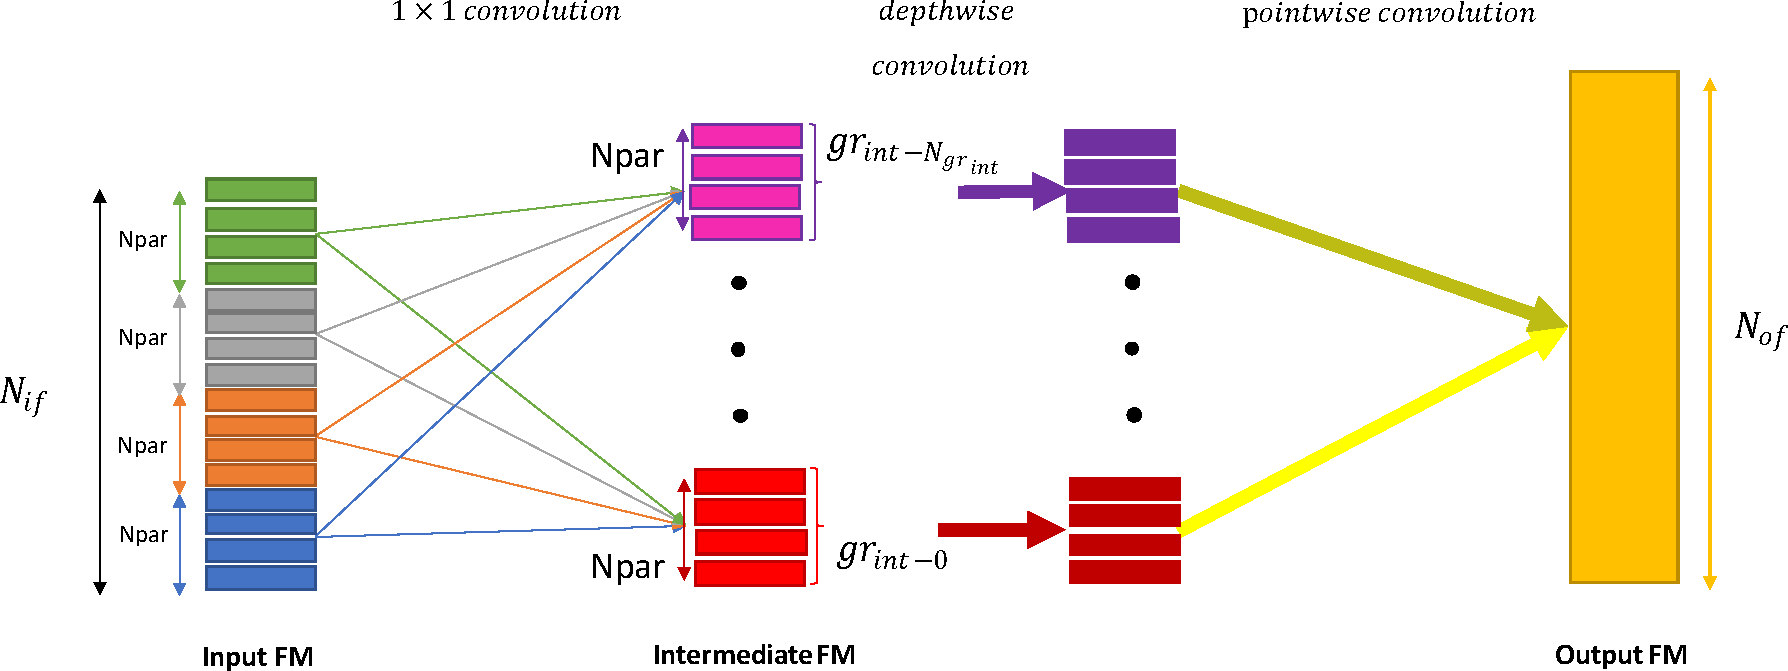
\includegraphics[width=\textwidth]{algo.pdf}
    \caption{Illustration of the algorithm used to perfom the convolutions}
    \label{fig:algo}
\end{figure}
%
As explained in Section \ref{subsec:pscheme}, each $1 \times 1$ convolution has to fetch $N_{par}$ input pixels, which corresponds to $N_{par}$ channels. Consequently, if the expansion $1 \times 1$ convolution produces $N_{par}$ channels, the \acrshort{dsc} can fetch those intermediate products and produce partial results of the output \acrshort{fm}. Indeed, we can first perform the depthwise convolution with each intermediate channel and then perform the partial pointwise convolution with the corresponding weight in each pointwise kernel, as illustrated in Figure \ref{fig:algo}.
The output \acrshort{fm} is computed when the \acrshort{dsc} has performed these steps for each intermediate group. This approach was chosen, instead of producing directly each final output result, to reuse at most the products of the $1 \times 1$ convolution.

\begin{algorithm}
    \centering
    \begin{algorithmic}
        \For{$group_{int}:=0$; $group_{int} < Ngr_{int}$; $group_{int}++$}
            \State{1*1\_convolution ($group_{int}$)}
            \State{DSC($group_{int}$);}
        \EndFor
    \end{algorithmic}
    \caption{Pseudocode of the algorithm}
    \label{pseudocode:overal_pseudo_code}
\end{algorithm}
%
We can translate this algorithm into a pseudocode, observed in Algorithm \ref{pseudocode:overal_pseudo_code}, where $group$ (respect. $group_{int}$) is the index of fetching group in the input \acrshort{fm} (resp. intermediate \acrshort{fm}, since the number of input channels is expanded by a factor $t$) and $Ngr_{int} = \left\lceil \frac{N_{if} \times t}{N_{par}} \right\rceil$ is the number of intermediate fetching groups. We can now detail how each convolution is going to be performed:

%
%
%
\begin{enumerate}
    \item \textbf{1*1\_convolution}: We have to fetch the $N_{par}$ kernels corresponding to the \acrshort{dsc} fetching group. Indeed, the \acrshort{dsc} needs to fetch $N_{par}$ channels of the intermediate \acrshort{fm}. Then we can perform the convolution. As described in Section \ref{subs:2dconv}, the kernel acts as a sliding window on the input \acrshort{fm}. For each pixel at position $(ix, iy)$, the convolution loads iteratively each weight and pixel fetching group in the channel-axis. For each fetching group $group \leq N_{group}$, the convolution is performed by multiplying each non-pruned weight with its corresponding pixel and accumulates the multiplication with the result of the previous group. The process is finished when the $N_{par}$ intermediate \acrshort{fm} channels have been produced (of size $N_{ix} \times N_{iy}$). The corresponding pseudocode is found in Algorithm \ref{pseudocode:c11} and the process is shown in Figure \ref{fig:algo_11conv}.
    \begin{algorithm}[H]
        \centering
        \begin{algorithmic}
            \For{$int_{f}:=0$; $int_{f} < N_{par}$; $int_{f}++$} \Comment{Loop 3}
                \For{$int_{x}:=0$; $int_{x} < N_{ix}$; $int_{x}++$} \Comment{Loop 2}
                    \For{$int_{y}:=0$; $int_{y} < N_{iy}$; $int_{y}++$} \Comment{Loop 2}
                        \For{$group:=0$; $group < N_{gr}$; $group++$} \Comment{Loop 1}
                            \For{$i_f:=0$; $i_f < N_{np}$; $i_f++$} \Comment{Unrolled}
                                \State{$wgt$  = $filter_{1 \times 1}$[$group_{int} \times N_{par} + int_f$][$group \times N_{np} + i_f$]}
                                \State{$acti$  = $FMI_{I}$[$wgt[pos] + group \times N_{par}$][$int_y$][$int_x$]}
                                \State{FM$_{int}$[$group_{int} \times N_{par} + int_f$][$int_y$][$int_x$]  += $acti \times wgt[val]$}
                            \EndFor
                        \EndFor
                    \EndFor
                \EndFor
            \EndFor
        \end{algorithmic}
        \caption{Sparse $1 \times 1$ convolution pseudocode}
        \label{pseudocode:c11}
    \end{algorithm}
    %
    \begin{figure}[H]
        \centering
        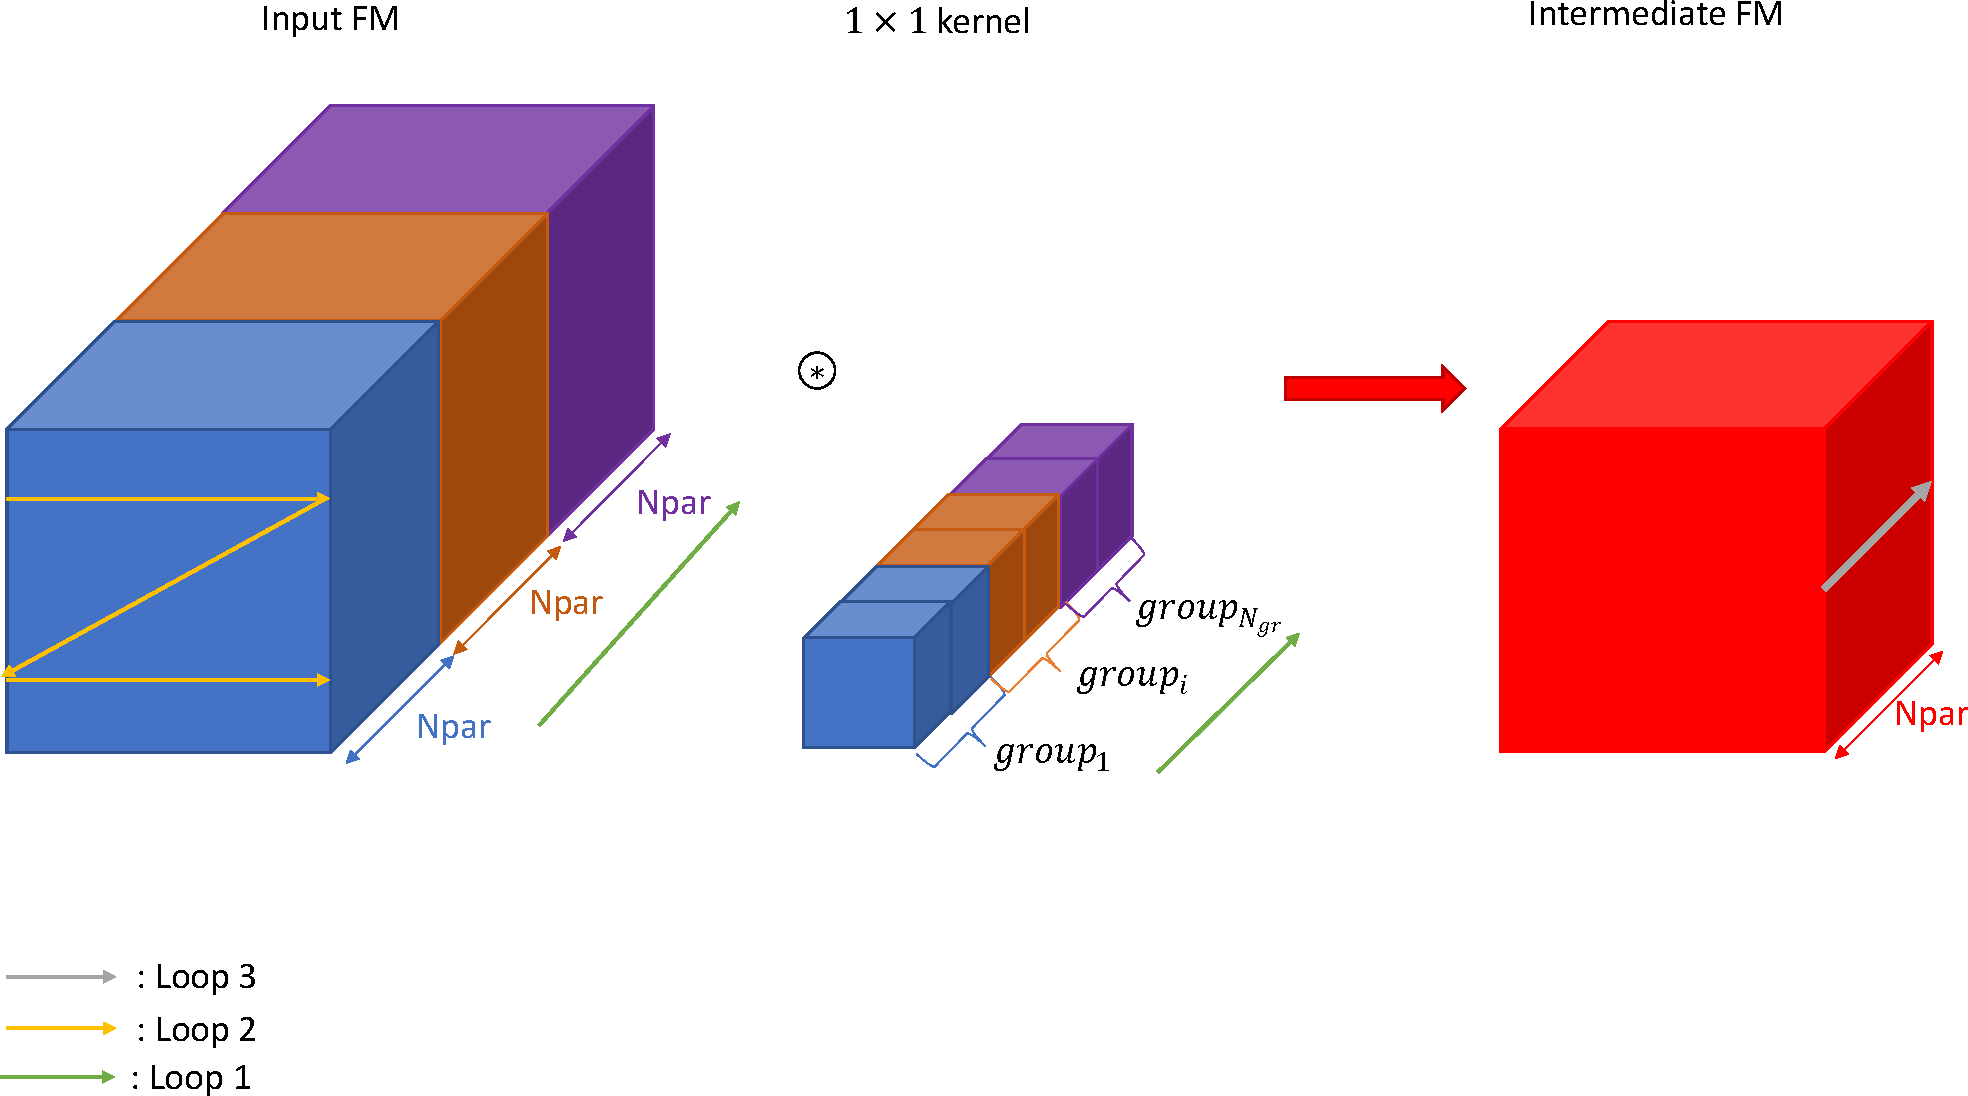
\includegraphics[width=\linewidth]{algo_c11.pdf}
        \caption{representation of the sparse $1 \times 1$ convolution}
        \label{fig:algo_11conv}
    \end{figure}
    %
    \item \textbf{\acrshort{dsc}} Once the $1 \times 1$ convolution has produced the next $N_{par}$ intermediate \acrshort{fm} channels, we can do the depthwise convolution with these channels. Once the depthwise convolution is done, we can fetch the corresponding weight fetching group in each of the pointwise filters and compute the partial results for each of the output \acrshort{fm} and sum them with the previous partial results. The corresponding pseudocode is found in Algorithm \ref{pseudocode:dsc} and the process is shown in Figure \ref{fig:algo_dsc}. We note that we have to add padding pixels since spatial dimensions are only reduced using stride $S$ (see Section \ref{subs:2dconv}).
    %
    \begin{algorithm}[H]
        \centering
        \begin{algorithmic}
            \For{$o_{y}:=0$; $o_{y} < N_{oy}$; $o_{y}++$} \Comment{Loop 4}
                \For{$o_{x}:=0$; $o_{x} < N_{ox}$; $o_{x}++$} \Comment{Loop 4}
                    \State{\% Depthwise convolution}
                    \For{$int_{f}:=0$; $int_{f} < N_{par}$; $int_{f}++$} \Comment{Loop 3}
                        \For{$k_{y}:=0$; $k_{y} < N_{ky}$; $k_{y}++$} \Comment{Loop 2}
                            \For{$k_{x}:=0$; $k_{x} < N_{kx}$; $k_{x}++$} \Comment{Loop 2}
                                    \State{FM$_{Dw}$[$group_{int} \times N_{par} + int_f$][$o_y$][$o_x$]  += }
                                    \State{FM$_{int}$[$group_{int} \times N_{par} + int_f$][$o_{y} \times S + k_{y}$][$o_{x} \times S + k_{x}$] $\times$} \State{kernel$_{dw}$[$group_{int} \times N_{par} + int_f$][$k_{y}$][$k_{x}$]}
                            \EndFor
                        \EndFor
                    \EndFor
                    \State{\% Pointwise convolution}
                    \For{$o_f:=0$; $o_f < N_{of}$; $of++$} \Comment{Loop 1}
                        \For{$i_f:=0$; $i_f < N_{np}$; $i_f++$} \Comment{Unrolled}
                            \State{$wgt$  = $filter_{Pw}$[$o_f$][$group_{int} \times N_{np} + i_f$]}
                            \State{$acti$  = $FMI_{Dw}$[$wgt[pos] + group_{int} \times N_{par}$][$o_y$][$o_x$]}
                            \State{FM$_{o}$[$o_f$][$o_y$][$o_x$] += $acti \times wgt[val]$}
                        \EndFor
                    \EndFor
                \EndFor
            \EndFor
        \end{algorithmic}
        \caption{Sparse \acrshort{dsc} convolution pseudocode}
        \label{pseudocode:dsc}
    \end{algorithm}
    %
    \begin{figure}[H]
        \centering
        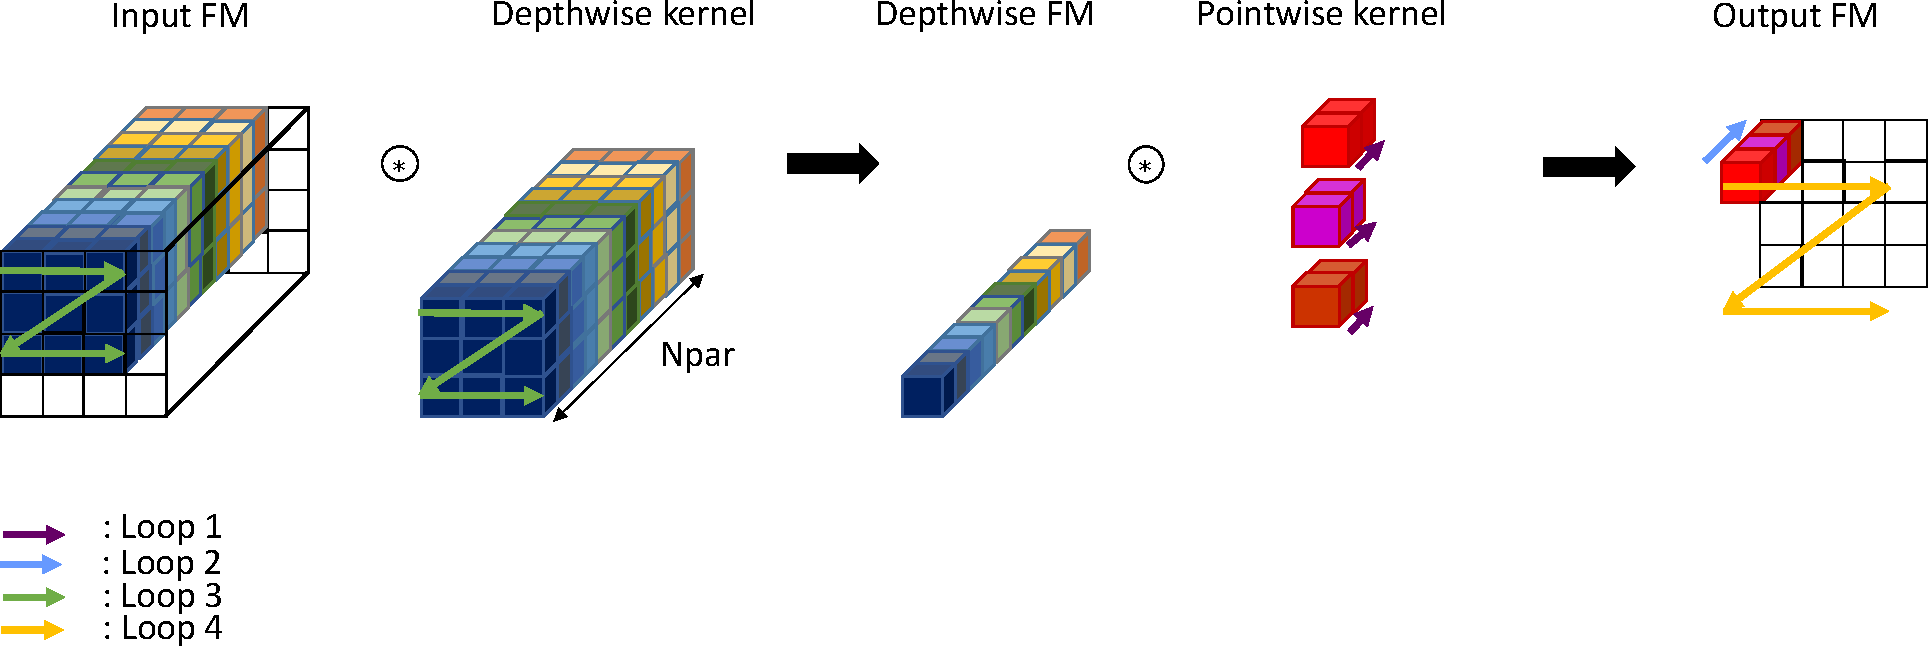
\includegraphics[width=\linewidth]{algo_dsc.pdf}
        \caption{representation of the sparse \acrshort{dsc} convolution}
        \label{fig:algo_dsc}
    \end{figure}
\end{enumerate}
%
\subsection{Loop analysis}
%
Once we have determined how the convolutions are going to be performed, we can now define how it will be implemented on \acrshort{fpga}. As explained in Section \ref{sec:opti_dataflow}, the \acrshort{cnn} inference is executed in three repeated steps:
%
\begin{enumerate}
    \item The \acrshort{fpga} loads a tile of the data from the external memory into the on-chip memory.
    \item The \acrshort{pe}s of the \acrshort{fpga} fetch data from the on-chip memory, use them to perform convolution, and store the computed result into the on-chip memory.
    \item Once the tile of output results is produced, it is stored into the external memory. Either the \acrshort{fpga} loads the next tile and restarts the operations, either it stops if the last tile of data has been convolved.
\end{enumerate}
%
If we look at Algorithm \ref{pseudocode:c11} and \ref{pseudocode:dsc}, each convolution is implemented with various levels of loop. To optimize the loop operations, we can use tree main loop optimization techniques, as presented in Section \ref{sec:opti_dataflow}: loop tiling, loop unrolling, and loop interchange. Those loop optimization techniques include hardware design parameters that define the acceleration factor and hardware footprint \cite{ma_optimizing_2018}. Therefore, we have to analyse the convolution loops in order to find the optimal tiling, unrolling and loop interchange parameters. We are going to apply the same methodology as \textcite{ma_optimizing_2018}. However, as they studied the standard convolution, in this work we adapt it to the sparse \acrshort{dsc}.

\textcite{ma_optimizing_2018} identified design objectives to optimize the convolution operation. These following design objectives should be minimized:
%
\begin{itemize}
    \item Partial sum storage.
    \item On-chip memory accesses and data reutilisation.
    \item Off-chip memory accesses.
\end{itemize}
%
We will try to minimize them for both $1 \times 1$ and depthwise separable convolution.
%
\subsubsection{Hardware design parameters}
%
Before analyzing the design objectives, we must first define what are the different tiling and unrolling parameters for each convolution. In Table \ref{tab:param_c11} and Table \ref{tab:param_dsc} are defined the different dimensions of the volums and the hardware design parameters.

\textbf{$1 \times 1$ convolution}: the $1 \times 1$ convolution is composed of three convolution loops (the fourth loop is fully-unrolled according to the algorithm). During the first loop, we fetch each fetching group and we do the convolution between them. The first loop is determined by the number of input and weight fetching groups (they are the same since otherwise there would be misalignement). The purpose of the first loop is to compute the output final result of the convolution. The second loop slides spatially the kernel over the input \acrshort{fm} to produce one channel of the intermediate \acrshort{fm}. Since the spatial size of each kernel is $1 \times 1$, there is no spatial reduction between the input and intermediate \acrshort{fm}. The purpose of the third loop is to produce the required $N_{par}$ intermediate \acrshort{fm} channels.
%
\begin{table}[H]
    \centering
    \begin{tabular}{c|c|c|c}
    \hline \hline
    & \makecell{\# of weight \\ and input \\ fetching group} & \makecell{Input \acrshort{fm} \& \\ Output \acrshort{fm} \\ Spatial Axis} & \makecell{Output \acrshort{fm} \\ channels} \\
    \hline
    Convolution Loops & Loop-1 & Loop-2 & Loop-3 \\
    Convolution Dimensions & $N_{gr}$ & $N_{ix}$,$N_{iy}$ & $N_{par}$ \\
    Loop Tiling            & $T_{gr}$ & $T_{ix}$,$T_{iy}$ & $T_{intf}$ \\
    Loop Unrolling         & $P_{gr}$ & $P_{ix}$,$P_{iy}$ & $P_{intf}$ \\
    \hline \hline
    \end{tabular}
    \caption{$1 \times 1$ convolution loop dimensions and hardware design variables, inspired from \cite{ma_optimizing_2018}}
    \label{tab:param_c11}
\end{table}
%
\textbf{\acrshort{dsc}}: the \acrshort{dsc} is composed of four convolution loops. Two loops are specific to the depthwise convolution, one to the pointwise convolution and one loop is shared between the two convolutions. As presented in Section \ref{subsec:mbnv2-pr}, the pointwise convolution uses the output pixels of the depthwise convolution to produce the $N_{of}$ partial results in order to avoid reperforming the same $1 \times 1$ and depthwise convolution. Loop-1 therefore aims at looping over the output channels. The depthwise convolution is composed of two loops. Loop-2 performs the 2D convolution between the input channel and the corresponding kernel and Loop-3 loops over the input channel. Finally, Loop-4 is the one that selects which output pixels to compute and fetches the associated input pixels chunk of data from the on-chip memory.
%
\begin{table}[H]
    \centering
    \begin{tabular}{c|c|c|c|c|c}
    \hline \hline
    & \makecell{Output \acrshort{fm} \\ channels} & \makecell{Pointwise kernel \\ size} & \makecell{Input \acrshort{fm} \\ channels} & \makecell{Input \acrshort{fm} \\ Spatial Axis} & \makecell{Output \acrshort{fm} \\ Spatial Axis} \\
    \hline
    \makecell{Convolution \\ Loops}     & Loop-1   & Loop-2            & Loop-3     & Loop-4            & Loop-4 \\
    \makecell{Convolution \\ Dimensions}  & $N_{of}$ & $N_{kx}$,$N_{ky}$ & $N_{par}$  & $N_{ix}$,$N_{iy}$ & $N_{ox}$,$N_{oy}$\\
    \makecell{Loop \\ Tiling}          & $T_{of}$ & $T_{kx}$,$T_{ky}$ & $T_{intf}$ & $T_{ix}$,$T_{iy}$ & $T_{ox}$,$T_{oy}$\\
    \makecell{Loop \\ Unrolling}          & $P_{of}$ & $P_{kx}$,$P_{ky}$ & $P_{intf}$ & $P_{ix}$,$P_{iy}$ & $P_{ox}$,$P_{oy}$\\
    \hline \hline
    \end{tabular}
    \caption{\acrshort{dsc} loop dimensions and hardware design variables, inspired from \cite{ma_optimizing_2018}}
    \label{tab:param_dsc}
\end{table}
%
\subsubsection{Partial Sum Storage}
%
\textbf{$1 \times 1$ convolution}: In order to minimize the partial sum storage, we have to keep all partial results in the registers. If we store those partial results into the on-chip or off-chip memory, it would result in less efficiency in terms of energy consumption and latency. The optimal solution would be to fully unroll Loop-1. However, two problems arise. First, since the \acrshort{fpga} has constrained resources, it would not be feasible on the target platform. Second, the number of fetching groups vary accross the layers since it depends on the number of input channels ($N_{gr} = \frac{N_{if}}{N_{par}}$). We should adapt the unrolling parameter $P_{gr}$ to the worst case and there would be inefficiency problems. Indeed, if $N_{gr} < P_{gr}$, some \acrshort{pe} would not be used. A better solution would be to fully buffer each fetching group and keep the partial results in the registers. Therefore, we should compute Loop-1 first (otherwise some results would be stored in the on-chip memory).
In summary, the number of partial sums is determined by the number of $1 \times 1$ convolution \acrshort{pe}s in parallel, as shown in Equation \eqref{eq:psum_c11}. Each $1 \times 1$ convolution \acrshort{pe} can operate in parallel $P_{gr}$ fetching groups. To minimize the storage of partial sum, we should add the following constraint $T_{gr} = N_{gr}$. Moreover, the ratio of $P_{gr}$ to $N_{gr}$ should be an integer to avoid these inefficiency problems.
%
\begin{equation}
    \# psum = P_{ix} \times P_{iy} \times P_{intf}
    \label{eq:psum_c11}
\end{equation}

\textbf{\acrshort{dsc}}: during the \acrshort{dsc}, we can find two kinds of partial sums: the partial depthwise result and the partial output result. According to the proposed algorithm, we can not keep the partial output in the registers since we produce at each new fetching group every possible partial output results. It means that we have to keep the tile of output \acrshort{fm} in the on-chip memory as partial results, as illustrated in Equation \eqref{eq:psum_o_dsc}. Since the kernel size is small and constant accross the network, we can fully unroll Loop-2 and set $P_{kx} = T_{kx} = N_{kx}, P_{ky} = T_{ky} = N_{ky}$. This approach was also chosen by \textcite{motamedi_placid_2017}. Since the fetching group size $N_{par}$ is up to the programmer, we can also fully unroll Loop-3 $P_{intf} = T_{intf} = N_{par}$. As the depthwise convolution is fully unrolled, we can determine the number of depthwise partial sums using equation \ref{eq:psum_dw_dsc}.
%
\begin{equation}
    \# psum_{DSC_{PW}} = T_{ox} \times T_{oy} \times T_{of}
    \label{eq:psum_o_dsc}
\end{equation}
%
\begin{equation}
    \# psum_{DSC_{DW}} = N_{kx} \times N_{ky} \times N_{par}
    \label{eq:psum_dw_dsc}
\end{equation}
%
\subsubsection{On-chip memory accesses}
%
According to \textcite{ma_optimizing_2018}, the number of on-chip accesses is determined by Equation \eqref{eq:onchipaccess}, where $\#read_{px}$ (resp. $\#read_{wg}$) is the number of reads in the on-chip memory accesses for input pixel (resp. weight), $\#read\_write\_psum$ is the number of write and read accesses if we store partial sum in the on-chip memory, and  $\#write\_px$ is the number of accesses to write the output results (which is equal to the number of output pixels). Therefore, to reduce on-chip memory accesses, we have to limit partial sums stored in on-chip memory and limit the number of reads.
The number of reads can be reduced by reusing the data in the registers, and can be expressed using Equation \ref{eq:read_on_px} and \ref{eq:read_on_wg} \cite{ma_optimizing_2018}, where $N_{op}$ is the total number of operations in a convolution. We can analyze for each convolution $Data\_Reuse_{px}$ and $Data\_Reuse_{wg}$.
%
\begin{align}
    \#On\_chip\_accesses &= \#read_{px} + \#read_{wg} \\ &+ \#read\_write\_psum + \#write\_px
    \label{eq:onchipaccess}
\end{align}
%
\begin{equation}
    \#read_{px} = \frac{N_{op}}{Data\_Reuse_{px}}
    \label{eq:read_on_px}
\end{equation}
%
\begin{equation}
    \#read_{wg} = \frac{N_{op}}{Data\_Reuse_{wg}}
    \label{eq:read_on_wg}
\end{equation}

\textbf{$1 \times 1$ convolution}: data reuse should be maximized to limit the number of on-chip memory accesses which are less efficient than register accesses. \textcite{ma_optimizing_2018} define two kinds of data reutilisation: spatial reuse (how many data are reused in one cycle) and temporal reuse (if a data can be reused in more than one cycle). Temporal data reuse is only possible if we compute Loop-2 first (we keep the same kernel for the pixels of a channel). However, since we compute Loop-1 first, this is not possible. To increase spatial data reuse, we must increase the parallelization and so the unrolling parameters, as illustrated in Equation \eqref{eq:px-d-reu} and \eqref{eq:wg-d-reu}, where $Data\_Reuse_{px}$ (resp. $Data\_Reuse_{wg}$) is the data reuse for input pixels (resp. weight).
%
\begin{equation}
    Data\_Reuse_{px} = P_{intf}
    \label{eq:px-d-reu}
\end{equation}
\begin{equation}
    Data\_Reuse_{wg} = P_{ix} \times P_{iy}
    \label{eq:wg-d-reu}
\end{equation}

\textbf{\acrshort{dsc}}: Since Loop-3 and Loop-2 are fully unrolled, we have a full temporal data reuse for weight. The data reuse for pixel and weight for the depthwise convolution can be found in Equation \eqref{eq:px_dw-d-reu} \cite{ma_optimizing_2018} and \eqref{eq:wg_dw-d-reu}. For the pointwise convolution, we can avoid reading input pixels from on-chip memory. If we keep the $N_{par}$ results of the depthwise convolution in registers.
Using the same methodology as for \textbf{$1 \times 1$ convolution}, the weight data reuse can be expressed using Equation \eqref{eq:wg_pw-d-reu}
%
\begin{equation}
    Data\_Reuse_{px} = \frac{N_{kx} \times N_{ky} \times N_{par} \times P_{intx} \times P_{inty}}{\left( \left( P_{intx} - 1 \right)S + N_{kx} \right) \times \left( \left( P_{inty} - 1 \right)S + N_{ky} \right)}
    \label{eq:px_dw-d-reu}
\end{equation}
\begin{equation}
    Data\_Reuse_{wg-dw} = N_{kx} \times N_{ky} \times N_{par}
    \label{eq:wg_dw-d-reu}
\end{equation}
\begin{equation}
    Data\_Reuse_{wg-pw} = P_{ox} \times P_{oy}
    \label{eq:wg_pw-d-reu}
\end{equation}
%
\subsubsection{Off-chip memory accesses}
%
In the model presented in Section \ref{subsec:loopopti}, as the on-chip memory is not large enough to store the whole \acrshort{cnn} size, this one is stored in an external memory. However, accesses to the external memory are more expensive in terms of latency and energy. Therefore, we should limit the number of off-chip memory accesses per pixel and weight. Instead, we tile the weights and input \acrshort{fm} that we store in the on-chip memory. Once the tile has been fully used, we can load the next tile until the convolution is done.

%
\begin{figure}
    \centering
    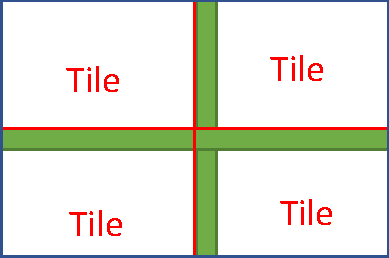
\includegraphics[width=\textwidth]{Tile.pdf}
    \caption{Tiling process on an input \acrshort{fm}, where the green area is the input pixels that would be loaded more than once due to 2D convolution}
    \label{fig:tilei}
\end{figure}
%
Since we store every pixel fetching group in the on-chip memory, each pixel should be loaded once from the external memory. However, if the tile does not cover the spatial size of the input \acrshort{fm}, due to the depthwise convolution, the input tile can be expressed as Equation \eqref{eq:tileo} \cite{ma_optimizing_2018}. It means that some pixels are included in multiple tiles, as illustrated in Figure \ref{fig:tilei}. Despite this, we can express the number of external memory accesses per pixel as Equation \eqref{eq:dram_px}.
%
\begin{equation}
    T_{ix/iy} = \left( T_{ox/oy} - 1\right) S + P_{kx/ky}
    \label{eq:tileo}
\end{equation}
\begin{equation}
    \#DRAM\_px = 1
    \label{eq:dram_px}
\end{equation}
%
If all the weights are not buffered into the on-chip buffer, we have to load from external memory the weight corresponding to the intermediate \acrshort{fm} fetching group. It means that we must fetch each weight everytime a new output tile is produced. Therefore, the number of weight external address is expressed as Equation \eqref{eq:dram_wg}.
%
\begin{equation}
    \#DRAM\_px = \frac{N_{ox} \times N_{oy}}{T_{ox} \times T_{oy}}
    \label{eq:dram_wg}
\end{equation}
%
\subsubsection{Summary}
%
After having analyzed the hardware design variables, we have determined each
%% tiling
%% unrolling
%% Loop interchange
